\documentclass[11pt,a4paper]{article}
\usepackage{iftex}
\ifPDFTeX
  \usepackage[T1]{fontenc}
  \usepackage[utf8]{inputenc}
\else
  \usepackage{fontspec}
\fi
\usepackage[spanish,es-noshorthands]{babel}
\usepackage{amsmath,amssymb}
\usepackage{booktabs}
\usepackage{graphicx}
\usepackage{geometry}
\usepackage{float}
\usepackage{hyperref}
\geometry{margin=2.4cm}
\graphicspath{{../results/tabla/graficas/}}
\hypersetup{colorlinks=true,linkcolor=black,urlcolor=blue}
\title{Informe de la reimplementación\\[0.35em]
\large Ondulaciones intrínsecas del grafeno, hasta $N=8640$}
\author{Emanuel Orozco Gallego}
\date{11 de noviembre de 2026}
\begin{document}
\maketitle

\begin{abstract}
Este informe explica, para quien no haya seguido la simulación, qué se copió del artículo de Fasolino, Los y Katsnelson (2007), qué se cambió a propósito y por qué las gráficas no son iguales a las del paper. La receta de Monte Carlo, las cajas y la temperatura de 300~K sí se reprodujeron. El potencial no es el del paper: es Tersoff, y por eso no aparece el pico agudo de unos 70~Å ni el comportamiento a 3500~K. Esa diferencia es la importante. El resto de las diferencias de las figuras son de dibujo o de un estimador distinto, y no cambian la lectura.
\end{abstract}

\section{De qué trata el trabajo}

El grafeno es una lámina de un átomo de espesor. Si se la deja libre, a temperatura ambiente no se queda plana: vibra y forma ondulaciones. El paper pregunta de qué tamaño son esas ondulaciones y si la teoría de una membrana elástica basta para explicarlas.

La respuesta del paper tiene dos capas. La primera es la de cualquier lámina flexible: las ondulaciones largas se frenan porque, al doblarse, la hoja también se estira. La segunda es propia del carbono: un enlace puede dejar de ser el enlace conjugado habitual (1.42~Å) y acercarse a un enlace doble (1.31~Å) o simple (1.54~Å). Ese cambio empuja los átomos fuera del plano y, según el paper, fija un tamaño preferido de unos 70~Å.

La simulación de aquí repite el experimento numérico del paper a 300~K, en todas las cajas de su Tabla~I que tienen como máximo 8640 átomos. Sirve para ver qué parte de la historia sale de la receta de Monte Carlo y de una lámina de carbono, y qué parte exige el detalle químico que el paper usa y aquí no está.

\section{Palabras que aparecen en las gráficas}

\begin{itemize}
\item \textbf{Monte Carlo.} Se propone un movimiento al azar. Si la energía baja, se acepta. Si sube, se acepta solo a veces, con una probabilidad que depende de la temperatura. Al cabo de muchos intentos, la hoja representa el equilibrio térmico.
\item \textbf{Un paso.} Son $N$ intentos, uno por átomo en promedio. $N$ es el número de átomos.
\item $h$. Cuánto se levanta cada átomo respecto del plano medio. $h_{\mathrm{rms}}$ es el promedio cuadrático de esas alturas: un solo número para toda la hoja.
\item $q$. El inverso de un tamaño. Un $q$ pequeño es una ondulación larga; un $q$ grande es una ondulación corta. $q\approx 0.1$~Å$^{-1}$ corresponde a unos 70~Å, porque $2\pi/q\approx 70$.
\item $G(q)$. Cuánta ondulación hay de ese tamaño. En el paper y aquí se dibuja $G(q)/N$.
\item $G_0$. La curva que saldría si la hoja fuera un resorte ideal, sin el freno entre doblado y estiramiento. Baja como $1/q^2$.
\item $g(r)$. A qué distancias hay átomos vecinos. El primer pico es la longitud del enlace.
\end{itemize}

\section{Qué se copió tal cual, y por qué}

Si se cambia la receta, una diferencia con el paper puede ser un error de la receta y no un efecto físico. Por eso estas piezas se dejaron como en el artículo.

\begin{enumerate}
\item Se empieza con la hoja completamente plana, para no imponer una ondulación de antemano.
\item El movimiento es el de Metrópolis, a 300~K.
\item Un paso son $N$ intentos de mover una coordenada.
\item Cada cinco pasos se propone un cambio de área, igual en las dos direcciones de la caja. La hoja puede dilatarse o contraerse.
\item Hay $4\times 10^5$ pasos para llegar al equilibrio y $5\times 10^5$ para promediar.
\item Se miden $h$, $G(q)=q^2|h_q|^2$ y $g(r)$. La referencia $G_0$ usa la rigidez $\kappa=1.1$~eV del paper.
\end{enumerate}

Esas decisiones importan. Sin ellas, no se podría decir si una curva distinta es física o es otra simulación.

\section{Qué se cambió, y por qué}

\subsection{El potencial no es el del paper}

El paper evalúa la energía con LCBOPII. Ese potencial describe el carbono de forma que un enlace puede pasar de conjugado a parcialmente doble o simple, y ese cambio está ligado a la salida del plano.

LCBOPII no está disponible aquí como biblioteca. Se usó Tersoff en la parametrización de Lindsay y Broido, hecha para el grafeno. Es de la misma familia: la fuerza del enlace depende de los vecinos, y la distancia de equilibrio sigue siendo 1.42~Å. No tiene el canal de conjugación de largo alcance de LCBOPII.

Esta es la decisión de fondo. Con Tersoff se puede comprobar la receta, la caja, el enlace y la parte elástica de la ondulación. No se puede comprobar la afirmación central del paper: que el carbono fija un largo de unos 70~Å porque sus enlaces cambian de tipo. Reproducir el paper \emph{en esa afirmación} sí exigiría LCBOPII. Reproducirlo en el resto, no.

\subsection{Solo hasta 8640 átomos, y solo a 300~K}

La Tabla~I del paper tiene seis tamaños. El último, $N=19940$, queda por encima del tope que se pidió, así que no se simuló. Los otros cinco sí: 240, 960, 2160, 4860 y 8640. Hacen falta los cinco porque el paper compara las cajas pequeñas, donde no cabe una onda de 70~Å, con las grandes, donde sí cabe.

La temperatura de 3500~K (Figs.~4 y~5 del paper) no se simuló. El protocolo pedido es 300~K. Además, a 3500~K el paper ve que el máximo se corre a unos 30~Å y que $g(r)$ abre hombros en 1.31 y 1.54~Å. Eso es el mismo canal de conjugación, ahora con más energía térmica. Tersoff no abre esos hombros. Correr 3500~K con este potencial no produciría esas dos figuras.

\subsection{La caja de $N=960$}

La fórmula que cierra la Tabla~I es $L_x=p|a_1|$ y $L_y=q\cdot 3a$, con $a=1.42$~Å y $N=4pq$. Todas las filas coinciden con eso, menos el $L_x$ impreso de $N=960$: la tabla dice 49.29~Å y la fórmula da 49.19~Å. Se simuló 49.19~Å, el valor coherente con las demás filas. La diferencia es 0.10~Å, menor que el efecto que se discute.

\subsection{Cómo se usó la máquina}

El cálculo es el mismo Metrópolis. Para que terminara en horas y no en días, los átomos que están lejos se mueven a la vez, y cada tamaño usa un reparto de núcleos que llena los 64 del equipo: desde 64 copias de la caja pequeña hasta 2 copias de las cajas grandes, con más hilos cada una. Una copia de más en la caja grande da una barra de error más ancha. En $N=8640$, $h_{\mathrm{rms}}$ sale $0.47\pm 0.07$~Å precisamente porque solo hay dos copias. Eso no cambia la física de cada copia.

\section{Qué salió}

\begin{center}
\small
\begin{tabular}{rrrrrr}
\toprule
$N$ & $h_{\mathrm{rms}}$ (Å) & $E/N$ (eV) & pico de $g(r)$ (Å) & $G/G_0$ & $q$ mínimo \\
\midrule
240  & $0.180\pm 0.007$ & $-7.939$ & 1.435 & 0.73 & 0.243 \\
960  & $0.318\pm 0.021$ & $-7.939$ & 1.435 & 0.74 & 0.121 \\
2160 & $0.385\pm 0.016$ & $-7.938$ & 1.435 & 0.74 & 0.081 \\
4860 & $0.473\pm 0.025$ & $-7.939$ & 1.445 & 0.75 & 0.054 \\
8640 & $0.470\pm 0.075$ & $-7.939$ & 1.445 & 0.75 & 0.040 \\
\bottomrule
\end{tabular}
\end{center}

$E/N$ es la energía por átomo. En la hoja plana de este Tersoff vale $-7.966$~eV. El valor de la tabla, $-7.939$~eV, está un poco por encima, como corresponde a una hoja tibia, y es el mismo en los cinco tamaños. El primer pico de $g(r)$ cae junto a 1.42~Å. $G/G_0$ cerca de 0.75, en la zona de $q$ intermedia, dice que la definición de $G(q)$ y la rigidez de 1.1~eV son las del paper. La aceptación de los movimientos de átomo fue del 39~\% en todos los tamaños: el paso al azar no está ni congelado ni aceptándolo todo.

$h_{\mathrm{rms}}$ crece con el lado de la caja y luego se frena. Una membrana elástica ideal crecería en línea recta con el lado. Quedar por debajo de esa recta es el freno entre doblado y estiramiento, que el paper también discute. Para $N=8640$ el paper cita una altura típica de unos 0.6~Å, mirando la figura. Aquí el número es la raíz cuadrática media, 0.47~Å. Son el mismo orden. No son el mismo estimador, y no hace falta que coincidan al segundo decimal.

\begin{figure}[H]
\centering
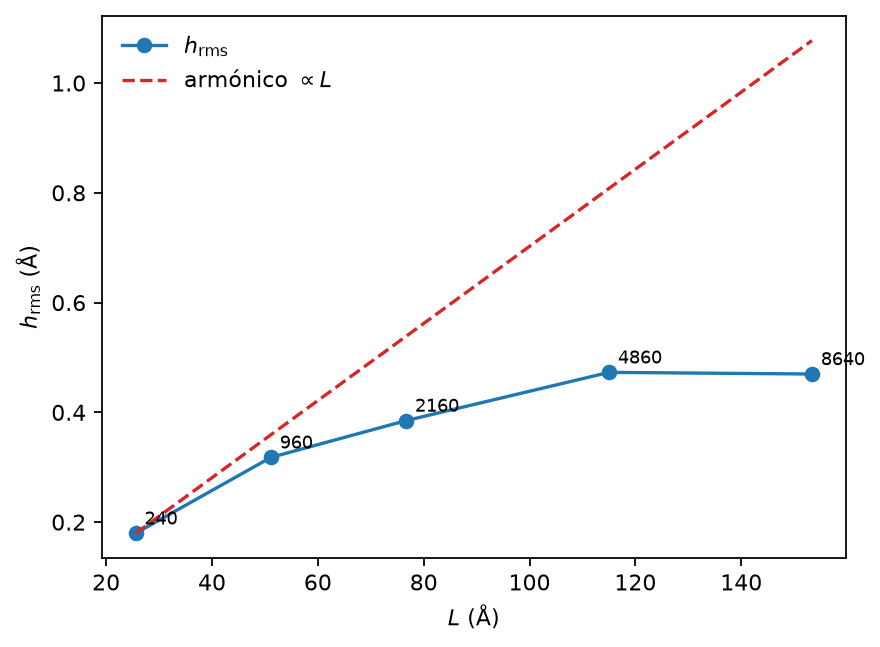
\includegraphics[width=0.78\textwidth]{hrms_vs_L.png}
\caption{Altura media de la hoja frente al lado largo de la caja. La recta roja es el crecimiento de una membrana elástica ideal, anclado en la caja más pequeña. Los puntos se quedan por debajo: las ondulaciones largas se frenan.}
\end{figure}

\section{Por qué las gráficas no son las del paper}

\subsection{La curva de $G(q)$}

\begin{figure}[H]
\centering
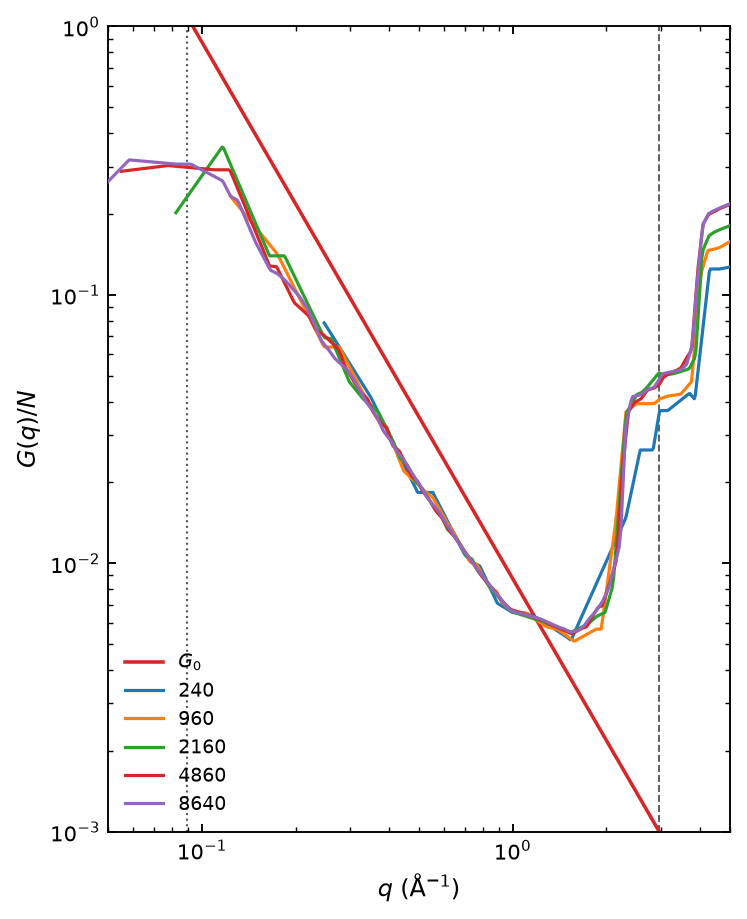
\includegraphics[width=0.62\textwidth]{Gq_fig3.png}
\caption{$G(q)/N$ de las cinco cajas, en los mismos ejes que la Fig.~3 del paper: $q$ de 0.05 a 5~Å$^{-1}$ y $G/N$ de $10^{-3}$ a 1. La recta roja es $G_0$. La línea punteada marca los 70~Å. La discontinua marca el primer pico de Bragg, en 2.95~Å$^{-1}$.}
\end{figure}

Entre $q\sim 0.2$ y $q\sim 2$ las cinco curvas caen juntas, un poco por debajo de la recta roja. Esa parte sí es la del paper: ahí la aproximación armónica describe la hoja, y la convención de Fourier es la correcta.

A la izquierda, las cajas grandes dejan de subir como $1/q^2$. La caja de 240 átomos ni siquiera llega a esa zona: su lado es de unos 25~Å, así que la onda más larga que cabe está en $q=0.24$~Å$^{-1}$. El paper dice lo mismo de sus dos cajas más cortas que 70~Å. Hasta ahí, la figura se lee igual.

La diferencia está en la forma de ese apartamiento. El paper dibuja un máximo agudo cerca de $q\approx 0.1$~Å$^{-1}$ y lo atribuye a la conjugación de LCBOPII. Aquí se ve una meseta ancha, y de una copia a otra el valor se mueve tanto como la propia bajada. No es ese pico. Llamarlo igual sería afirmar un resultado que el potencial no puede dar. La meseta sí importa: muestra el freno anarmónico. El pico agudo de 70~Å importaría si la pregunta fuera la del paper sobre el enlace químico. Con Tersoff, esa pregunta queda sin contestar, y es correcto que la gráfica no finja el pico.

\subsection{Los dos picos de la derecha}

En la Fig.~3 del paper, a la derecha hay dos agujas. Están en $q=2.95$~Å$^{-1}$ y $q=5.11$~Å$^{-1}$. Son los picos de Bragg: las direcciones en las que la red del grafeno se repite. No son la ondulación de 70~Å. Cualquier hoja de grafeno los tiene, salga o no el efecto de conjugación.

En los datos de esta simulación esas direcciones también están, y son muy intensas. En la caja de 8640 átomos, el modo más alto cerca del primer Bragg llega a $G/N\approx 500$, y cerca del segundo pasa de 5000. La curva de la figura no los dibuja como agujas porque no es el modo más alto: es la mediana de las miles de direcciones que tienen un $|q|$ parecido. Casi todas son ondulación térmica ordinaria (mediana 0.05 y 0.24). Unas pocas, las de la red, se disparan. La mediana cuenta la mayoría.

El borde derecho del eje es $q=5$, el mismo marco que se midió en la figura del paper. El segundo pico, en 5.11, cae justo ahí. Aunque se alargara el eje, la altura no sería la del paper: allí las agujas llegan cerca de 1, y aquí los modos de Bragg salen del marco por arriba. Dibujar dos picos de altura 1 sería copiar el dibujo, no los números. Para la pregunta de las ondulaciones largas, esos picos no son lo que hay que igualar. Sí confirman que la red es grafeno.

\subsection{La distancia entre vecinos}

\begin{figure}[H]
\centering
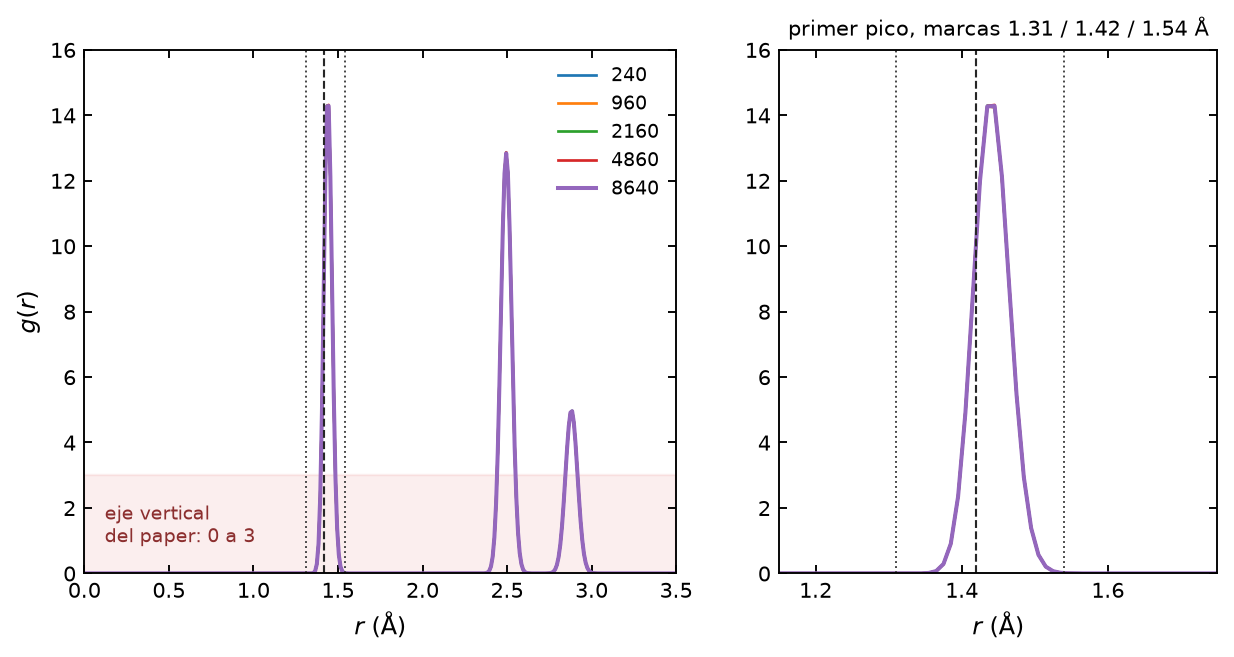
\includegraphics[width=0.92\textwidth]{rdf_fig5.png}
\caption{Distancia entre átomos, con el mismo eje horizontal que la Fig.~5 del paper (0 a 3.5~Å). Las marcas son 1.31, 1.42 y 1.54~Å. La banda rosa es la altura del eje vertical del paper, de 0 a 3. El pico de la simulación llega cerca de 14 porque el intervalo de la cuenta es de 0.01~Å.}
\end{figure}

El primer pico cae en 1.44~Å, al lado del enlace conjugado de 1.42~Å. No hay hombros en 1.31 ni en 1.54~Å. Esos hombros, en el paper, aparecen sobre todo a 3500~K y son la firma de enlaces doble y simple. Aquí no están porque el potencial no abre ese canal y porque esa temperatura no se corrió.

La altura del pico no se compara con la del paper. El paper llega cerca de 3 en un eje etiquetado ``rdf''. Aquí $g(r)$ está normalizada para valer 1 a distancia grande, y el pico es estrecho (unas cinco centésimas de ångström). Un pico estrecho, contado en intervalos de 0.01~Å, sale alto. Lo que se compara es la posición. Los picos siguientes, cerca de 2.46 y 2.84~Å, están donde el paper también tiene vecinos.

\subsection{La foto de la hoja}

\begin{figure}[H]
\centering
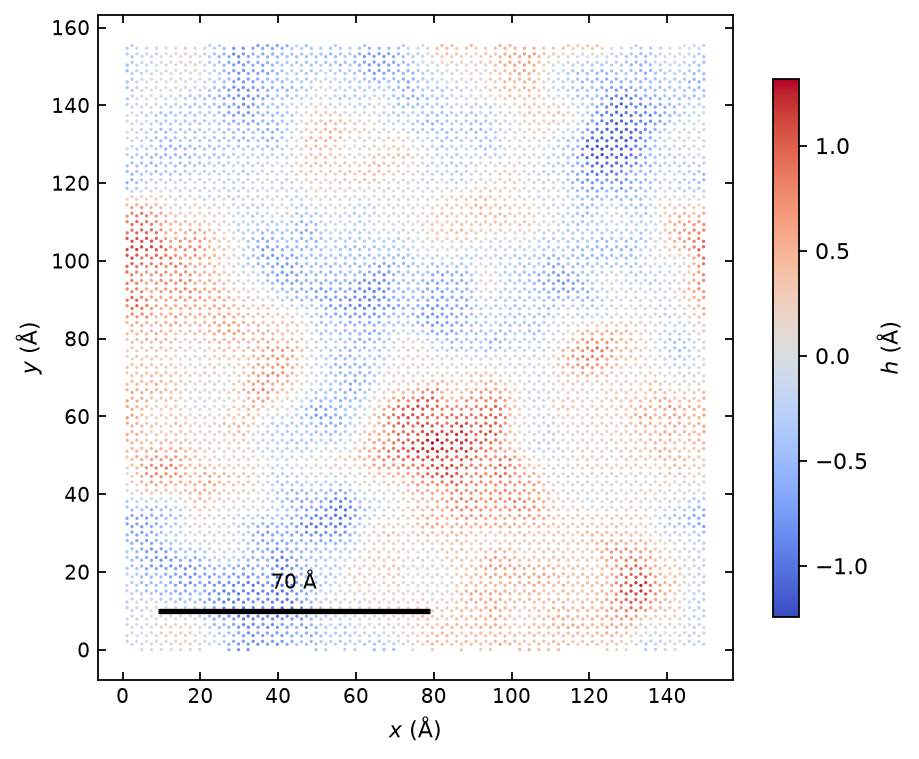
\includegraphics[width=0.72\textwidth]{snapshot_fig1.png}
\caption{La hoja de 8640 átomos a 300~K, vista desde arriba. La barra negra mide 70~Å, la misma longitud que el paper dibuja sobre su Fig.~1. El color es la altura $h$.}
\end{figure}

Una instantánea en tres dimensiones se veía, al principio, como una hoja arrugada. No lo estaba. El programa igualaba el eje vertical al tamaño de la caja, y 2~Å de altura ocupaban en el dibujo lo mismo que 75~Å de lado. Las figuras nuevas amplían el eje vertical seis veces y lo dicen en el título. La barra de color sigue en ångströms reales, del orden de $\pm 1$~Å. Concuerda con $h_{\mathrm{rms}}$ de unas pocas décimas de ångström y con la altura típica de 0.6~Å que cita el paper.

\section{Qué sí haría falta igualar, y qué no}

Igualar la receta de Monte Carlo, las cajas, la temperatura de 300~K y la definición de $G(q)$ y de $g(r)$ sí importa. Sin eso, no se sabe si el programa hace el experimento del paper. Esa parte está hecha, y los números de la tabla la sostienen: el enlace, la energía, la aceptación y el tramo en que $G$ sigue a $G_0$.

Igualar el pico agudo de 70~Å, los hombros de $g(r)$ y el corrimiento a 30~Å a 3500~K también importa, pero para otra pregunta: la del enlace químico. Esa pregunta es la novedad del paper. No se responde con Tersoff, y no se responde alargando la simulación ni retocando la gráfica. Hace falta LCBOPII, y para las Figs.~4 y~5 hace falta además correr a 3500~K. Hasta entonces, lo honesto es mostrar la meseta y decir que no es el pico.

Igualar el dibujo de los dos picos de Bragg a altura 1 no importa para esa conclusión. Son la red cristalina. Están en los datos, en otras direcciones y con otra altura. Forzarlos en la curva mediana ocultaría la ondulación térmica, que es lo que la figura compara con $G_0$.

$N=19940$ alargaría la misma meseta a una caja mayor. Las tres cajas que ya superan 70~Å se parecen entre sí, así que el tope de 8640 átomos no es lo que borra el pico. Lo que lo borra es el potencial.

\section{Lectura corta}

La simulación hace el Monte Carlo del paper, a 300~K, en las cinco cajas de hasta 8640 átomos. La hoja se ondula, el enlace sigue en 1.42~Å, la energía es estable y, en los tamaños intermedios, $G(q)$ sigue la ley elástica del paper, un poco por debajo. Las ondulaciones dejan de crecer con el tamaño de la caja. Todo eso se ve en las gráficas y no depende de dibujarlas de otra forma.

Lo que no se ve, el máximo fino de 70~Å y el comportamiento a 3500~K, no faltó por un error de la corrida. Falta el canal de conjugación de LCBOPII. Copiar esas curvas sin ese potencial no acercaría la reimplementación al paper.
\end{document}
